%if __name__ == '__main__':
%    from numpy import std, average, sqrt, polyfit, log
%    from sqlite3 import connect
%    from os import environ
%
%    conn_1 = connect(environ['HOKU_PROJECT_PATH'] + '/data/lumberjack-all-triad.db')
%    cur = conn_1.cursor()
%
%    # 1,   2,      3,      4,      5,     6,    7,   8
%    # 0.0, 1.0e-6, 1.0e-5, 0.0001, 0.001, 0.01, 0.1, 1.0
%
%    for d in [[1, 2, 3, 4, 5, 6, 7, 8], [0.0, 1.0e-6, 1.0e-5, 0.0001, 0.001, 0.01, 0.1, 1.0]]:
%        t = polyfit(log(d[3:]), [0.9725, 0.386, 0.0035, 0.0, 0.0], 1)
%        print('Angle: {}*ln(x) + {}'.format(t[0], t[1]))
%
%        t = polyfit(log(d[4:]), [0.9885, 0.7055, 0.033, 0.00383333333333333], 1)
%        print('Dot: {}*ln(x) + {}'.format(t[0], t[1]))
%
%        t = polyfit(log(d[2:]), [0.9715, 0.8135, 0.259, 0.0253333333333333, 0.0095, 0.00716666666666667], 1)
%        print('Sphere: {}*ln(x) + {}'.format(t[0], t[1]))
%
%        t = polyfit(log(d[2:]), [0.9865, 0.8615, 0.332166666666667, 0.0245, 0.0095, 0.00483333333333333], 1)
%        print('Plane: {}*ln(x) + {}'.format(t[0], t[1]))
%
%        t = polyfit(log(d[3:]), [0.999333333333334, 0.354333333333333, 0.0, 0.0, 0.0], 1)
%        print('Pyramid: {}*ln(x) + {}'.format(t[0], t[1]))
%
%        t = polyfit(log(d[1:]), [1.0, 0.65, 0.0035, 0.0, 0.0, 0.0, 0.0], 1)
%        print('Composite: {}*ln(x) + {}'.format(t[0], t[1])), print()

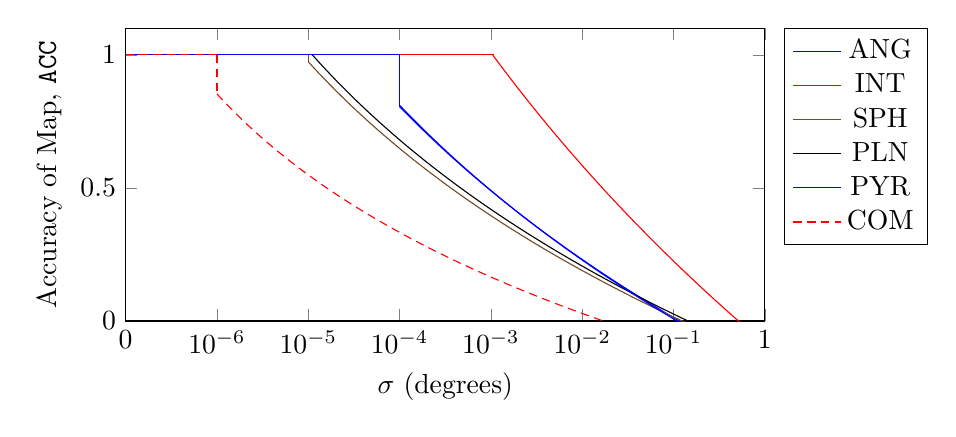
\begin{tikzpicture}
    \begin{axis}[
    width=0.8\linewidth, height=5.3cm,
    ylabel={Accuracy of Map, \texttt{ACC}}, ymin=0, ymax=1.1,
    xlabel={$\sigma$ (degrees)}, xmin=1, xmax=8,
    xtick={1, 2, 3, 4, 5, 6, 7, 8},
    xticklabels={$0$, $10^{-6}$, $10^{-5}$, $10^{-4}$, $10^{-3}$, $10^{-2}$, $10^{-1}$, $1$},
    samples=100, no markers, legend pos=outer north east, enlargelimits=false
    ]
        \addplot +[domain=1:4, forget plot]{1};
        \addplot +[forget plot] coordinates {(4, 1) (4, 0.8055384229041530)};
        \addplot +[domain=4:8]{-1.416887591459587*ln(x) + 2.7697617012853217};
        \addlegendentry{ANG}

        \addplot +[domain=1:5.03, forget plot]{1};
%        \addplot +[forget plot] coordinates {(5, 1) (5, 1)};
        \addplot +[domain=5.02:8]{-2.3292306442173216*ln(x) + 4.757244753386215};
        \addlegendentry{INT}

        \addplot +[domain=1:3, forget plot]{1};
        \addplot +[forget plot] coordinates {(3, 1) (3, 0.9738787471803161)};
        \addplot +[domain=3:8]{-1.1317828984553227*ln(x) + 2.217269347527745};
        \addlegendentry{SPH}

        \addplot +[domain=1:3, forget plot]{1};
%        \addplot +[forget plot] coordinates {(3, 1) (3, )};
        \addplot +[domain=3.04:8]{-1.1696544292494204*ln(x) + 2.301996347627258};
        \addlegendentry{PLN}

        \addplot +[domain=1:4, forget plot]{1};
        \addplot +[forget plot] coordinates {(4, 1) (4, 0.8105837347641904)};
        \addplot +[domain=4:8]{-1.4347255837709008*ln(x) + 2.7995357213002334};
        \addlegendentry{PYR}

        \addplot +[domain=1:2, forget plot]{1};
        \addplot +[forget plot] coordinates {(2, 1) (2, 0.8533960244900531)};
        \addplot +[domain=2:8]{-0.7510156659772902*ln(x) + 1.3739604159185614};
        \addlegendentry{COM}
    \end{axis}
\end{tikzpicture}